% nVSDguide.tex
% v4.0 released October 2014

\documentclass{nVSD2e}

\usepackage{epstopdf}% To incorporate .eps illustrations using PDFLaTeX, etc.
\usepackage{subfigure}% Support for small, `sub' figures and tables

\theoremstyle{plain}
\newtheorem{theorem}{Theorem}[section]
\newtheorem{corollary}[theorem]{Corollary}
\newtheorem{lemma}[theorem]{Lemma}
\newtheorem{proposition}[theorem]{Proposition}

\theoremstyle{definition}
\newtheorem{definition}{Definition}

\theoremstyle{remark}
\newtheorem{remark}{Remark}

\begin{document}

%\jvol{00} \jnum{00} \jyear{2014} \jmonth{October}

\articletype{RESEARCH ARTICLE}

\title{Design of a Feedback-Feedforward Steering Controller for Accurate Path Tracking and Stability at the Limits of Handling}

\author{
\name{Nitin R. Kapania $^{\rm a}$$^{\ast}$\thanks{$^\ast$Corresponding author. Email: nkapania@stanford.edu}, J. Christian Gerdes$^{\rm a}$}
\affil{$^{a}$Department of Mechanical Engineering, Stanford University, Building 550, Stanford, CA, 94305, phone: +16507244058}
\received{Received 00 Month 2015}
}

\maketitle

\begin{abstract}

This paper presents a feedback-feedforward steering controller that simultaneously maintains vehicle stability at the limits
of handling while minimizing lateral path tracking deviation. The design begins by considering the performance of a baseline
controller with a lookahead feedback scheme and a feedforward algorithm based on a nonlinear vehicle handling diagram.
While this initial design exhibits desirable stability properties 
at the limits of handling, the steady-state path deviation increases significantly at highway speeds. 
Results from both linear and nonlinear analyses indicate that lateral path tracking deviations are minimized when vehicle sideslip 
is held tangent to the desired path at all times. Analytical results show that 
directly incorporating this sideslip tangency condition into the steering feedback dramatically improves lateral path tracking, 
but at the expense of poor closed-loop stability margins.  However, incorporating the desired sideslip behavior
into the feedforward loop creates a robust steering controller capable of accurate path 
tracking and oversteer correction at the physical limits of tire friction. Experimental data collected from an 
Audi TTS test vehicle driving at the handling limits on a full length race circuit demonstrates the improved performance of the final
controller design. 
\end{abstract}

\begin{keywords}Autonomous driving, vehicle dynamics and control, autonomous path following
\end{keywords}


% {\abstractfont\centerline{\bfseries Index to information contained in this guide}\vspace{12pt}
% \hbox to \textwidth{\hsize\textwidth\vbox{\hsize18pc
% \hspace*{-12pt} {1.}  Introduction\\
% \hspace*{7pt} {1.1.}  The {\it nVSD} document class\\
% \hspace*{7pt} {1.2.}  Submission of \LaTeX\ articles\\
% \hspace*{24pt}        to the journal\\
% {2.}    Using the {\it nVSD} class file\\
% {3.}    Additional features\\
% \hspace*{10pt}{3.1.}  Title, authors' names, abstract\\
% \hspace*{24pt}        and keywords\\
% \hspace*{10pt}{3.2.}  Additional footnotes to the\\
% \hspace*{24pt}        title or authors' names\\
% \hspace*{10pt}{3.3.}  Lists\\
% {4.}    Some guidelines for using\\
% \hspace*{6pt}        standard features\\
% \hspace*{10pt}{4.1.}  Sections\\
% \hspace*{10pt}{4.2.}  Illustrations (figures)\\
% \hspace*{10pt}{4.3.}  Tables\\
% \hspace*{10pt}{4.4.}  Landscape pages\\
% \hspace*{10pt}{4.5.}   Theorem-like environments\\
% \noindent \hspace*{7pt} {4.6.}   Typesetting mathematics\\
% \hspace*{24pt} {4.6.1.}  Displayed mathematics\\
% \hspace*{24pt} {4.6.2.}  Bold math italic symbols\\
% \hspace*{24pt} {4.6.3.}  Bold Greek\\
% \hspace*{24pt} {4.6.4.}  Upright Greek characters  \\
% \hspace*{47pt}             and the upright partial \\
% \hspace*{47pt}             derivative sign  \\}
% \hspace{-24pt}\vbox{\noindent\hsize18pc
% \hspace*{7pt} {4.7.}   Acknowledgements \\
% \hspace*{7pt} {4.8.}   Funding \\
% \hspace*{7pt} {4.9.}   Notes \\
% \hspace*{7pt} {4.10.}   Supplemental material \\
% \hspace*{7pt} {4.11.}   References \\
% \hspace*{24pt} {4.11.1.}   References cited in the \\
% \hspace*{52pt}            text\\
% \hspace*{24pt} {4.11.2.}   The list of references\\
% \hspace*{7pt} {4.12.}   Appendices \\
% {5.}    Example of a section heading \\*
% \hspace*{6pt}   including {\fontencoding{T1}\scshape{small caps}}, {\it italic}, \\
% \hspace*{6pt}   and bold Greek such as ${\bm\kappa}$ \\
% {6.}    {\it nVSD} journal style \\
% \hspace*{10pt}{6.1.}   Hyphens, en rules, em rules \\ \hspace*{27pt}and minus signs\\
% \hspace*{10pt}{6.2.}   References \\
% \hspace*{10pt}{6.3.}   Maths fonts\\
% {7.}    Troubleshooting\\
% {8.}    Fixes for coding problems\\
% {9.}    Obtaining the nVSD2e class file\\
% \hspace*{10pt}{9.1}  Via the Taylor \& Francis \\
% \hspace*{24pt}       website\\
% \hspace*{10pt}{9.2}   Via e-mail\\\\}}}


\section{Introduction}
\label{sec:intro}

Improvements in the cost and performance of real-time sensing and embedded computing have resulted in a proliferation
of autonomous vehicle technology over the last two decades. A central control task in the operation of an autonomous vehicle is the ability
to maneuver along a desired path, typically generated by a high-level path planner. As a result, a significant research effort has been devoted to the subject of active steering control for autonomous or semi-autonomous vehicles.

In particular, steering systems based on feedback-feedforward control architectures have been a major focus of research.
Early work by Shladover et al. \cite{shladover} described a feedforward steering control law where the steady-state
steering angle was determined from path curvature and longitudinal force inputs. The feedback steering algorithm was linear state feedback on lateral path deviation, heading deviation and their
derivatives. The feedback gains were selected using a frequency shaped linear quadratic (FSLQ) algorithm to minimize
 path tracking error while maintaining good ride quality at different frequencies. Nagai et al. \cite{nagai} also used linear quadratic 
regulation to design two feedback steering controllers for autonomous path following, with one controller using steer angle as the control input
and the other using steering torque. 

Another approach for implementing the feedback-feedforward control architecture is robust ($H_\infty$) control synthesis.
Mammar and Koenig \cite{mammar} describe a driver-in-the-loop active handling system relying on results from robust
 control theory to minimize deviation from a desired trajectory. The steering feedback acts on the yaw rate error as opposed to path tracking error, and utilizes a feedforward action that is a function of the
 driver steering command. An improved steering assistance system was later presented by Raharijaona et al. \cite{raharijaona} 
 with an added torque input to improve stability margins. 

Finally, a simple but effective approach to feedback-feedforward steering control is to design a controller with the objective of
making the lateral tracking error zero at a certain `lookahead' point in front of the vehicle. Minimization of a lookahead
objective was studied by Hingwe and Tomizuka \cite{hingwe}, who proposed an input-output linearization controller to achieve this objective.
A crucial result from this study was the finding that internal yaw dynamics can be damped at all longitudinal velocities by making the
lookahead point a quadratic function of the vehicle velocity. Rosseter \cite{rosseter} also studied lookahead feedback systems extensively,
and derived a similar controller by seeking to minimize a quadratic potential function of the projected lookahead error. 

Regardless of the control strategy, ensuring passenger safety in emergency safety maneuvers requires that autonomous steering 
systems achieve both stability and accurate tracking of a reference path at the physical limits of tire adhesion. Autonomous path-following at the limits of handling has therefore become an actively explored topic of research. Kritiyikarana
 and Gerdes \cite{mickcop} developed a steering controller on an Audi TTS with lookahead steering feedback and a feedforward approach based on
 tracking the vehicle center of percussion. This controller performed well at high levels of lateral acceleration (7-8 $\mathrm{m/s^2}$),
 but experienced significant vehicle oscillations near the limits of handling. In related work, Talvala et al.  \cite{talvala} examined the Lyapunov stability of lookahead feedback
at the limits of handling, and determined that desirable stability properties were maintained
even in the presence of significant front and rear tire saturation. 

More recently, Filho and Wolf \cite{filho14} presented simulation results for a front-wheel steering controller based on dynamic model inversion. The resulting controller was able to track a reference oval path at the friction limits, and responded well
to added curvature discontinuities. Carvalho et al. \cite{carvalho13} demonstrated a nonlinear model predictive controller (MPC) 
capable of steering an experimental passenger sedan around obstacles at high speeds on an icy road. The controller was based 
on a nonlinear Ackermann model that was iteratively linearized. Yang et al. \cite{yang14} proposed a closed-loop Quasi-Linear Optimal Controller (QLOC) to reduce the post-collision lateral path deviation of a vehicle
in a traffic accident. The robustness properties of the controller were demonstrated in simulation on a high-fidelity multi-body vehicle model. Finally, Sharp \cite{sharp10} developed a linear optimal preview controller
for motorcycle path tracking at the cornering limits. Gain scheduling according to speed and lateral acceleration enabled a range of linear controllers to be applied in different driving conditions.
 
 This paper presents the design of a feedback-feedforward steering controller capable of combined stability and accurate path tracking at the limits of handling. 
 A baseline controller with lookahead steering feedback and feedforward based on the nonlinear handling diagram is presented in Section 2. 
Section 3 uses steady-state simulation results to demonstrate the relatively poor path tracking performance of this baseline. In Section 4, the authors 
consider a modifed steering feedback that aims to keep the vehicle sideslip tangent to the desired path, resulting in a closed-loop steering
response with zero steady-state lateral path deviation, but at the cost of poor stability margins. A better design approach, presented in Section 5, is to incorporate the desired sideslip behavior
as a feedforward input, which significantly improves path tracking while maintaining robust stability margins. Section 6 provides experimental data collected
on an Audi TTS test vehicle at Thunderhill Raceway in Willows, California, with combined lateral and longitudinal accelerations up to 9.5 $\mathrm{m/s^2}$.

\section{Controller Architecture}
\label{sec:controller}

A block diagram of a typical feedback-feedforward structure for steering control is shown in Fig.~\ref{fig:controllerBD}. Inputs to the feedforward
steering $\delta_\mathrm{FFW}$ are the current path curvature $\kappa$ and forward velocity $U_\mathrm{x}$. Inputs to the feedback steering $\delta_\mathrm{FB}$ are lateral path deviation
$e$ and path heading error $\Delta\Psi$ (Fig.~\ref{fig:bikeModel}b). The total steering command $\delta$ is the sum of the feedback and feedforward inputs.

% % % % % % % figure, blockdiagram % % % % % % %
\begin{figure}[h]
\centering
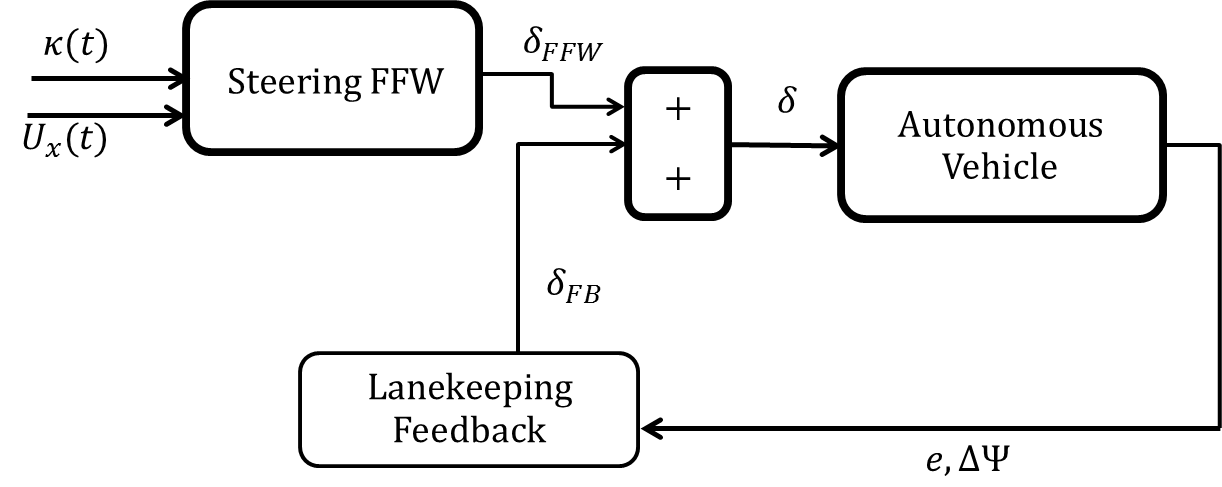
\includegraphics[width=.75\columnwidth]{figures/FB_FFW.png}
\caption{Block diagram of feedback-feedforward steering controller.}
\label{fig:controllerBD}
\end{figure}
% % % % % % % end figure % % % % % % %

For the purposes of this work, the desired path curvature for the vehicle to follow is provided to the controller via a separate path planning algorithm \cite{theodosis}. 
Additionally, the velocity profile is obtained from a longitudinal controller that keeps the combined vehicle acceleration 
magnitude at a specified value \cite{mickcop}.

\subsection{Feedforward Steering Design}
\label{sec:baselineFFW}

The objective of the steering feedforward is to provide an estimate of the steer angle required to traverse a path with a known path curvature and velocity profile.
This minimizes the level of compensation required by the steering feedback, reducing tracking errors and allowing for less overall control effort. 
To simplify the controller structure, the feedforward steering angle should depend only on the desired trajectory and be independent of the actual vehicle states.

The proposed structure of the steering feedforward begins with the assumption that vehicle dynamics are given by the planar bicycle model,
 with relevant vehicle states and dimensions shown in Fig.~\ref{fig:bikeModel}(a). 
This assumption allows the feedforward algorithm to account for the basic vehicle
 steering behavior while leaving roll and weight transfer effects to be handled by the steering feedback. 

\begin{figure}[h]
\centering
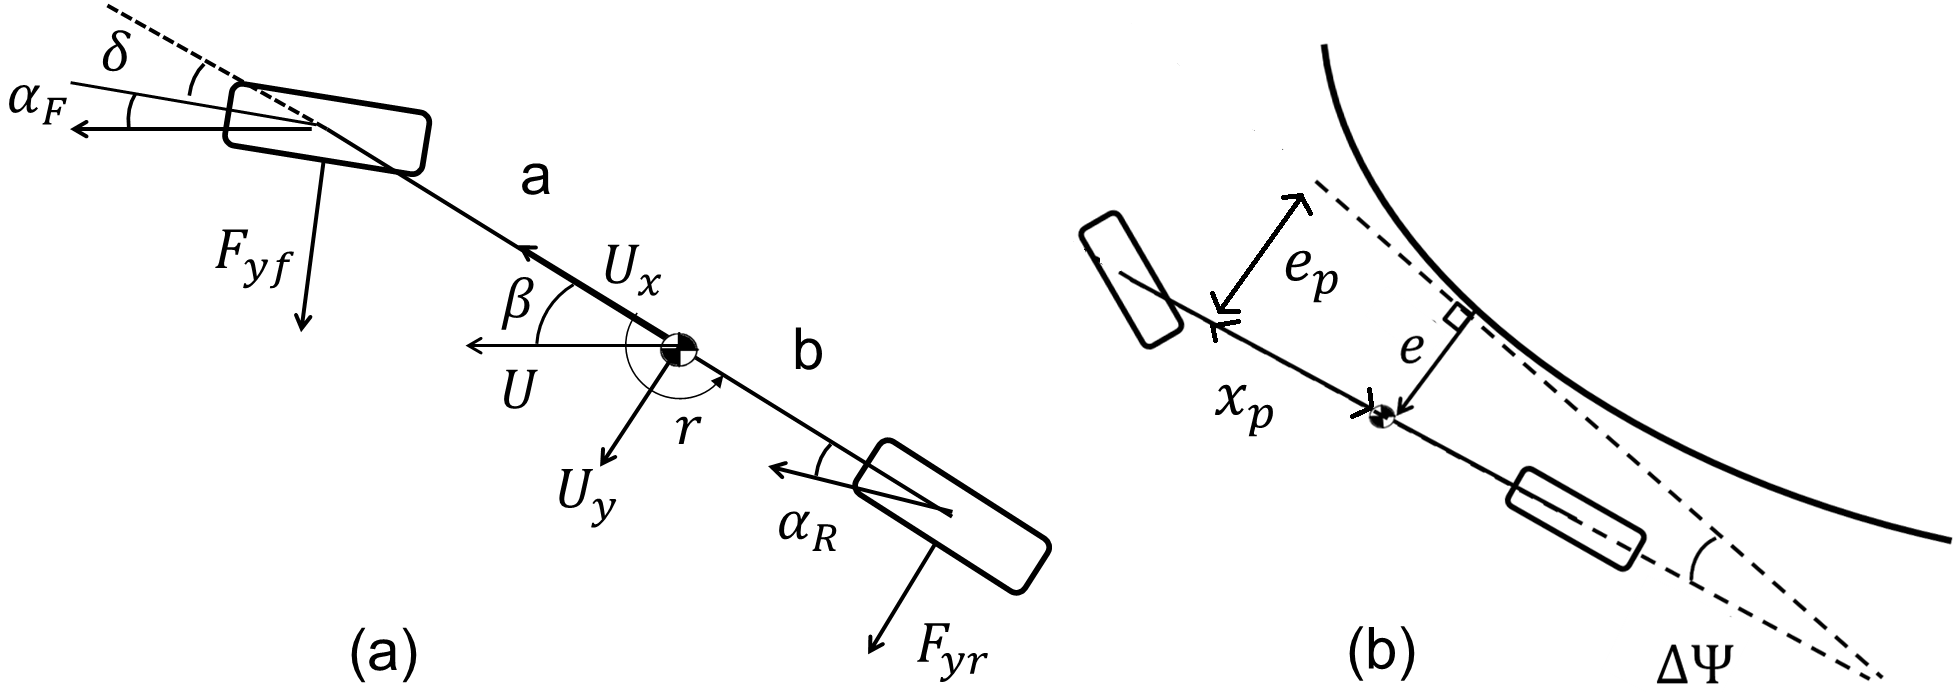
\includegraphics[width=.9\columnwidth]{figures/BikeModelSchematic.png}
\caption{ (a) Schematic of planar bicycle model (b) Projected error $e_p$ for feedforward steering calculation.}
\label{fig:bikeModel}
\end{figure}

The problem of determining suitable feedforward lateral tire forces for autonomous path following was studied by Krisada and Gerdes \cite{mickcop}. The (linearized) equations of 
motion for the states shown in Fig.~\ref{fig:bikeModel} are given by:

\begin{subequations}
\label{eq:bm}
\begin{align}
	\dot{\beta} &= \frac{F_\mathrm{yf}+F_\mathrm{yr}}{mU_x} - r \label{eq:bm1}\\
	\dot{r} &= \frac{aF_\mathrm{yf} - bF_\mathrm{yr}}{I_z} \label{eq:bm2} \\
	\dot{e} &= U_x (\beta + \Delta\Psi) \label{eq:bm3} \\
	\Delta\dot{\Psi} &= r - \dot{s}\kappa \label{eq:bm4} 
\end{align}
\end{subequations}
where $m$ and $I_z$ are the vehicle mass and out-of-plane rotational inertia, and $s$ is the distance along the desired path. Taking time derivatives of $\dot{e}$ and $\Delta\dot{\Psi}$ and substituting from (\ref{eq:bm1}) and (\ref{eq:bm2}) yields:
\begin{subequations}
\label{eqn:doubleds}
\begin{align}
	\ddot{e} &= \frac{F_\mathrm{yf}+F_\mathrm{yr}}{m} - U_x\kappa\dot{s} \\
	\Delta\ddot{\Psi} &= \frac{aF_\mathrm{yf} - bF_\mathrm{yr}}{I_z} -\kappa\ddot{s} - \dot{\kappa}\dot{s}
\end{align}
\end{subequations}
In general, the values chosen for the feedforward front and rear tire forces $F_\mathrm{yf}$ and $F_\mathrm{yr}$ should
bring $\ddot{e}$ and $\Delta\ddot{\Psi}$ to zero. However, for a typical front-steer vehicle, 
direct control is only available for the front steering force $F_\mathrm{yf}$ via command of the steering input $\delta$. The rear tire
force depends indirectly on the front steering angle via the build-up of rear tire slip $\alpha_\mathrm{r}$. It is therefore
not possible to simultaneously eliminate both the lateral tracking error and heading angle error. 

An alternative is to consider eliminating a weighted combination of the two error states by eliminating the lateral tracking 
error $e_p$ at a specified point $x_p$ in front of the vehicle, as shown in Fig.~\ref{fig:bikeModel}b. The error dynamics at this projected point are given by: 

\begin{subequations}
\label{eqn:xp}
\begin{align}
	e_p        &= e + x_\mathrm{p}\Delta\Psi \\
	\ddot{e}_p &= \frac{F_\mathrm{yf} + F_\mathrm{yr}}{m} - U_\mathrm{x}\kappa\dot{s} + x_p\frac{aF_\mathrm{yf} - bF_\mathrm{yr}}{I_z} - x_p(\kappa\ddot{s} + \dot{\kappa}\dot{s})
\end{align}
\end{subequations}

Kritayakirana and Gerdes \cite{mickcop} proposed the center of percussion $x_\mathrm{cop} = \frac{I_z}{bm}$ as a convenient projection point
for the feedforward steering. Substituting $x_p = x_\mathrm{cop}$ and $\ddot{e}_\mathrm{cop} = 0$  yields a simplified equation for the front tire force:

\begin{equation}
\label{eqn:xcop}
 F_\mathrm{yf} = \frac{mb}{L}(U_\mathrm{x}^2\kappa + x_\mathrm{cop}(\kappa\ddot{s} + \dot{\kappa}\dot{s}))
\end{equation}

The benefit of choosing the center of percussion becomes clear in (\ref{eqn:xcop}). The error dynamics at the
center of percussion are independent of the rear tire force, which can be highly transient when the vehicle is cornering near the
limits of handling. This leaves the only control input as $F_\mathrm{yf}$, which can be directly
manipulated by the front wheel steering. 

A feedforward steering approach based on eliminating tracking error at the center of percussion performed well experimentally at high lateral accelerations up to
7-8 $\frac{m}{s^2}$ \cite{mickcop}. However, at higher lateral accelerations, the closed-loop steering response became underdamped, and
the result was significant levels of yaw rate and steering wheel oscillation. This was due to the complex relationship between the 
desired feedforward front tire force $F^\mathrm{FFW}_\mathrm{yf}$ and the required steering angle $\delta_\mathrm{FFW}$ needed to achieve that desired tire force. 
In general, this relationship is dependent on the vehicle yaw rate $r$ and sideslip $\beta$:

\begin{equation}
\label{eqn:bikeffw}
\delta_\mathrm{FFW} = \frac{U_\mathrm{x}\beta + ar}{U_\mathrm{x}} - f^{-1}(F^\mathrm{FFW}_\mathrm{yf})
\end{equation}
where $f^{-1}(F_\mathrm{y})$ is an inverse tire model relating tire force to tire slip. Even though (\ref{eqn:xcop}) does not explicitly 
depend on  rear tire force, the feedforward steering command $\delta_\mathrm{FFW}$ implicitly depends on the transient
rear tire dynamics through the yaw rate and sideslip states. At the limits of handling, these transient dynamics become difficult to model.

To eliminate yaw rate oscillation, we propose simplifying the feedforward tire forces by assuming steady-state cornering conditions. Setting $\dot{s} = U_\mathrm{x}$, $\ddot{s} = \dot{\kappa} = 0$
in (\ref{eqn:xcop}) and $\dot{r} = 0$ in (\ref{eq:bm}) yields the following front and rear tire forces:

\begin{subequations}
\label{eqn:ffwforces}
\begin{align}
  F_\mathrm{yf}^\mathrm{FFW} = \frac{mb}{L} U_\mathrm{x}^2\kappa\\
   F_\mathrm{yr}^\mathrm{FFW}=\frac{ma}{L} U_\mathrm{x}^2\kappa
   \end{align}
\end{subequations}

At steady-state conditions and assuming small angles, the feedforward steering angle of the vehicle relates to the front and 
rear lateral tire slip $\alpha_\mathrm{f}$ and $\alpha_\mathrm{r}$ and vehicle yaw rate $r$ by vehicle kinematics:

\begin{equation}
\label{eqn:steadyffw}
\delta_{\mathrm{FFW}} = L\kappa - \alpha_\mathrm{f}^\mathrm{FFW}+\alpha_\mathrm{r}^\mathrm{FFW}
\end{equation}
where $\alpha_\mathrm{f}^\mathrm{FFW}$ and $\alpha_\mathrm{r}^\mathrm{FFW}$ are the lumped front and rear feedforward tire slip angles. The choice of feedforward 
tire slip angles is related to the tire forces in (\ref{eqn:ffwforces}) via the inverted tire model $f^{-1}(F_\mathrm{y})$. 
To account for saturation of tire force with increasing tire slip magnitude, a single friction coefficient brush Fiala model \cite{Pacejka2012} maps lateral 
tire slip angles into tire force as follows: 

\begin{eqnarray}
\label{eqn:fiala}
	F_\mathrm{y}&=&\begin{cases} -C_{\alpha}\tan\alpha + \frac{C_{\alpha}^2}{3\mu F_\mathrm{z}} |\tan\alpha| \tan\alpha - \frac{C_{\alpha}^3}{27\mu^2F_\mathrm{z}^2}\tan^3\alpha,
\hspace{4mm}  |\alpha| < \arctan{\left(\frac{3\mu F_\mathrm{z}}{C_\alpha}\right)} \\ -\mu F_\mathrm{z}\text{sgn} \ \alpha, \hspace{62mm} \mathrm{otherwise} \end{cases}
\end{eqnarray}
where $\mu$ is the surface coefficient of friction, $F_\mathrm{z}$ is the normal load, and $C_\alpha$ is the tire cornering stiffness. 
These parameters are determined from experimental data taken from a ramp-steer maneuver, as shown in Fig.~\ref{fig:tireCurve}.

\begin{figure}[h]
\centering
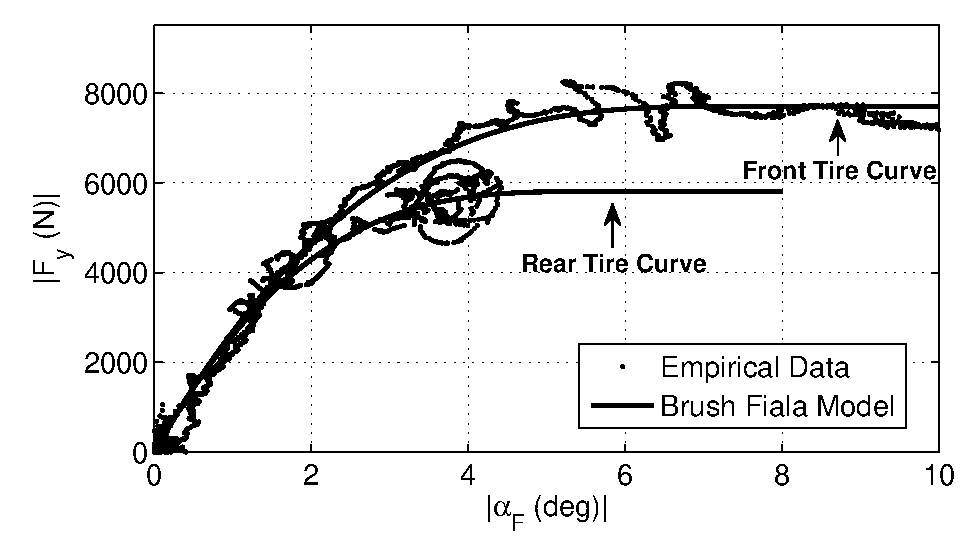
\includegraphics[width=0.85\columnwidth]{figures/FrontRearTireCurves.eps}
\caption{Nonlinear tire curves for FFW steering.}
\label{fig:tireCurve}
\end{figure}
\subsection{Feedback Steering Design}
\label{sec:lookahead}

With the feedforward design complete, the remaining step is to design the feedback controller. The goal of the feedback controller is to
minimize a `lookahead' error $e_\mathrm{LA}$, which is the vehicle tracking error projected a distance 
$x_\mathrm{LA}$ in front of the vehicle (Fig.~\ref{fig:lookaheadSchematic}).

\begin{figure}[h]
\centering
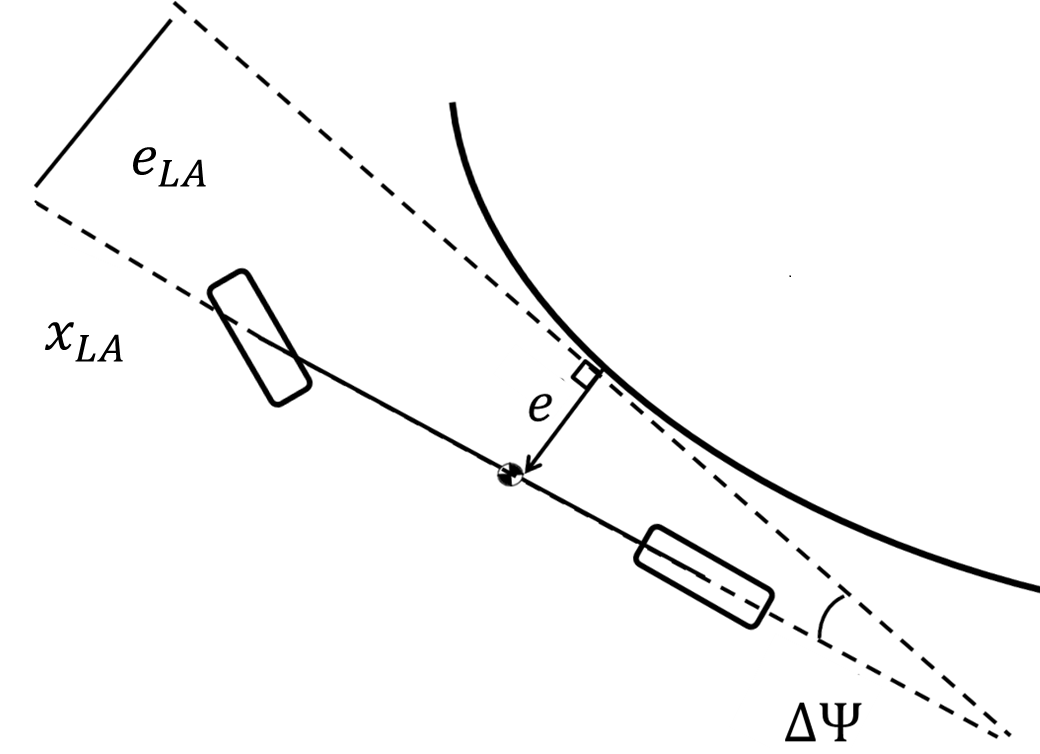
\includegraphics[width=.5\columnwidth]{figures/LookaheadSchematic.png}
\caption{Schematic of planar bicycle model showing projected lookahead error.}
\label{fig:lookaheadSchematic}
\end{figure}

The lookahead error and resulting feedback control law are given by:

\begin{subequations}
\label{eqn:lookahead}
\begin{align}
	e_\mathrm{LA}&=e+x_\mathrm{LA}\Delta\Psi \\
	\delta_\mathrm{FB} &= -k_\mathrm{P}e_\mathrm{LA}
\end{align}
\end{subequations}
with proportional gain $k_\mathrm{P}$. The control law (\ref{eqn:lookahead}) is a natural extension of potential field lanekeeping, as described by Rossetter et al. in \cite{rosseter}, which also provides heuristics for 
selecting $k_\mathrm{P}$ and $x_\mathrm{LA}$. Desirable stability properties over significant tire saturation levels are demonstrated in \cite{talvala}. 

\section{Predicted Steady-State Path Tracking Error}
\label{sec:predSS}

Simulation results provide useful insight about the steady-state path tracking behavior of the baseline feedback-feedforward system. 
Linearized equations of motion for the vehicle and error states can be written in state-space form, with state variable $x$ and control input $\delta$ defined as follows:

\begin{subequations}
\label{eqn:delta}
\begin{align}
		     x &= [e \hspace{2 mm} \Delta\Psi \hspace{2 mm} r \hspace{2 mm} \beta]^T \\
        \delta &=\delta_\mathrm{FB}+\delta_\mathrm{FFW} \\
               &=[-k_\mathrm{LK} \hspace{1 mm} -k_\mathrm{LK} x_\mathrm{LA} \hspace{3 mm} 0 \hspace{3 mm} 0] x+(L+\frac{K_\mathrm{ug} U_\mathrm{x}^2}{g}) \kappa
\end{align}
\end{subequations}
 where $K_\mathrm{ug}$ is the vehicle understeer gradient.
Note that $\delta_\mathrm{FB}$ in (\ref{eqn:delta}a) depends on the state variable, and $\delta_\mathrm{FFW}$ depends on the path curvature. Rewriting  
the vehicle state equations of motion using curvature as the input results in:

\begin{subequations}
\label{eqn:Amatrix}
\begin{align}
    \dot{x} &= Ax + B\kappa  \\
	A  &=  \begin{bmatrix}
   0 & U_\mathrm{x} & 0 & U_\mathrm{x} \\ 
   0 & 0 & 1 & 0 \\ 
   \frac{-ak_\mathrm{P} C_\mathrm{F}}{I_\mathrm{z}}  & \frac{-ak_\mathrm{P}x_{LA}C_\mathrm{F}}{I_\mathrm{z}}  & \frac{-(a^2C_\mathrm{F}+b^2C_\mathrm{R})}{U_\mathrm{x}I_\mathrm{z}} & \frac{bC_\mathrm{R} - aC_\mathrm{F}}{I_\mathrm{z}}  \\
   \frac{-k_\mathrm{P}C_\mathrm{F}}{mU_\mathrm{x}}  & \frac{-k_\mathrm{P}x_{LA}C_\mathrm{F}}{mU_\mathrm{x}}  & \frac{bC_\mathrm{R}-aC_\mathrm{F}}{mU_\mathrm{x}^2}-1 & \frac{-(C_\mathrm{F} + C_\mathrm{R})}{mU_\mathrm{x}}
  \end{bmatrix} \\
	B  &=[0 \hspace{2 mm} -U_\mathrm{x} \hspace{3 mm} \frac{a C_\mathrm{F} G_\mathrm{FFW}}{I_\mathrm{z}} \hspace{3 mm}  \frac{C_\mathrm{F} G_\mathrm{FFW}}{mU_\mathrm{x}}]^T
\end{align}
\end{subequations}
where $G_\mathrm{FFW} = (L+\frac{K_\mathrm{ug} U_\mathrm{x}^2}{g})$ and $C_\mathrm{F}$ and $C_\mathrm{R}$ are the lumped front and rear cornering stiffnesses. Fig.~\ref{fig:linError} shows results from using the linear model (\ref{eqn:Amatrix}) to compute steady-state path
 tracking errors over a range of vehicle speeds, given
 a constant lateral acceleration of $a_y =$ 3 $\mathrm{m/s}^2$. Additionally, steady-state results from the nonlinear feedforward control law 
 (\ref{eqn:steadyffw}) are plotted for the case where $a_y =$ 7 $\mathrm{m/s}^2$. For this high lateral acceleration case, the
 equations of motion (\ref{eq:bm}) and nonlinear Fiala tire model (\ref{eqn:fiala}) are used to predict the steady-state results. At low lateral accelerations, when the vehicle
 dynamics are dictated by linear equations of motion, the accumulated steady-state tracking error is small ($<$ .05 m) at highway speeds. However, 
when steering at the limits of handling, Fig.~\ref{fig:linError} shows that the increased sideslip of the vehicle results
 in higher steady-state tracking error, creating challenges for accurate driving in safety-critical situations. 
 
\begin{figure}[h]
\centering
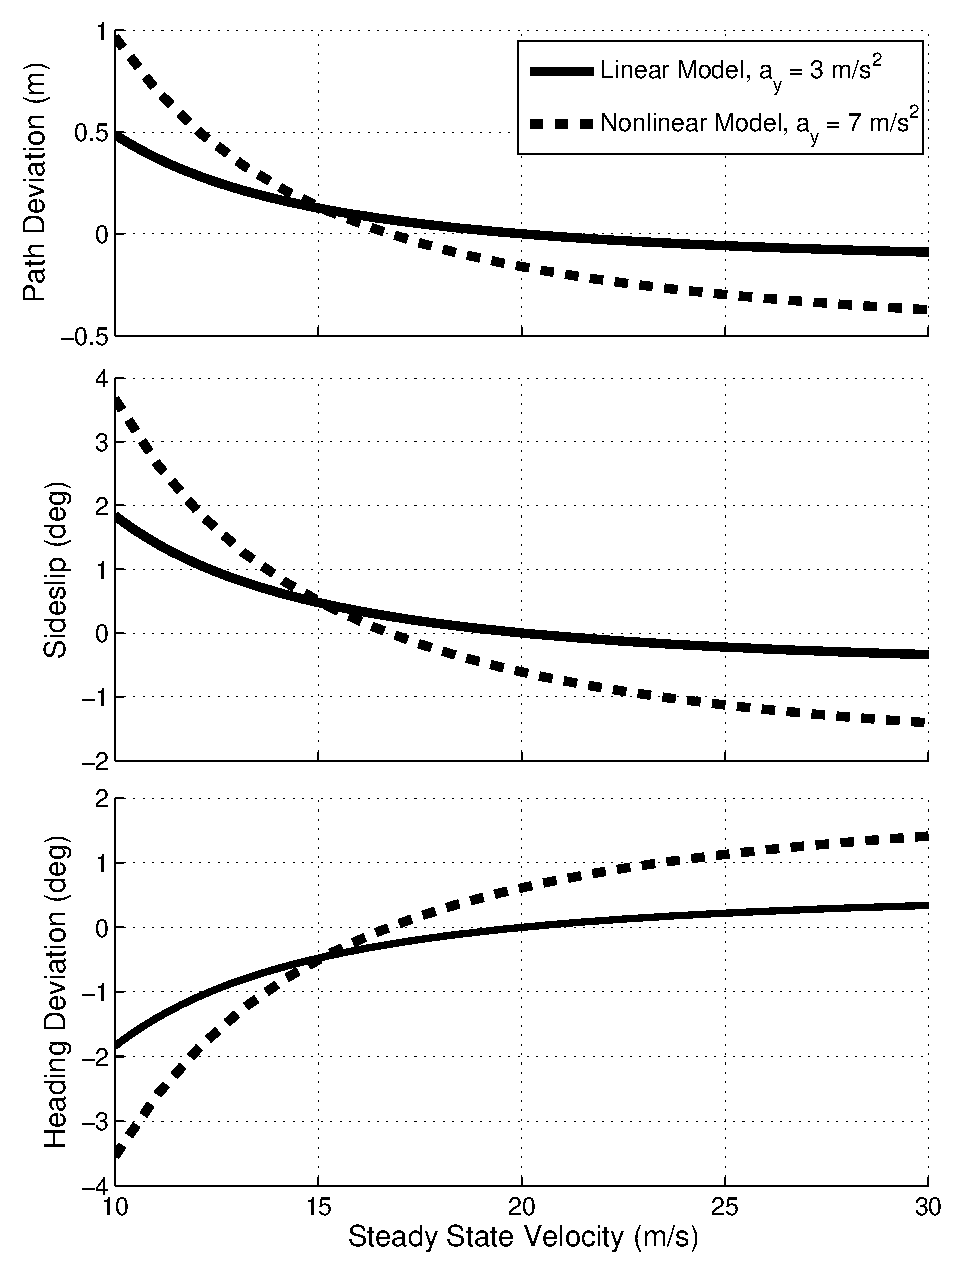
\includegraphics[width=.7\columnwidth]{figures/LinearErrorPlot.eps}
\caption{Steady-state path tracking error $e$, sideslip $\beta$ and heading deviation $\Delta\Psi$ as a function of vehicle speed. Results are plotted for the linear model, with fixed lateral acceleration $a_y = $ 3 $\mathrm{m/s}^2$, and for the
nonlinear model, with fixed lateral acceleration $a_y = $ 7 $\mathrm{m/s}^2$.}
\label{fig:linError}
\end{figure}
 
A qualitative explanation for this steady-state error is shown in Fig.~\ref{fig:SSerror}(a). Since the steering controller acts to eliminate a weighted
sum of heading error $\Delta\Psi$ and lateral path deviation $e$, the lookahead feedback is successful in
minimizing the desired metric $e_\mathrm{LA}$ at the projected distance $x_\mathrm{LA}$ in front of the vehicle. However, this still allows for steady-state equilibria where
values of $e$ and $\Delta\Psi$ themselves are nonzero.  

\begin{figure}[h]
\centering
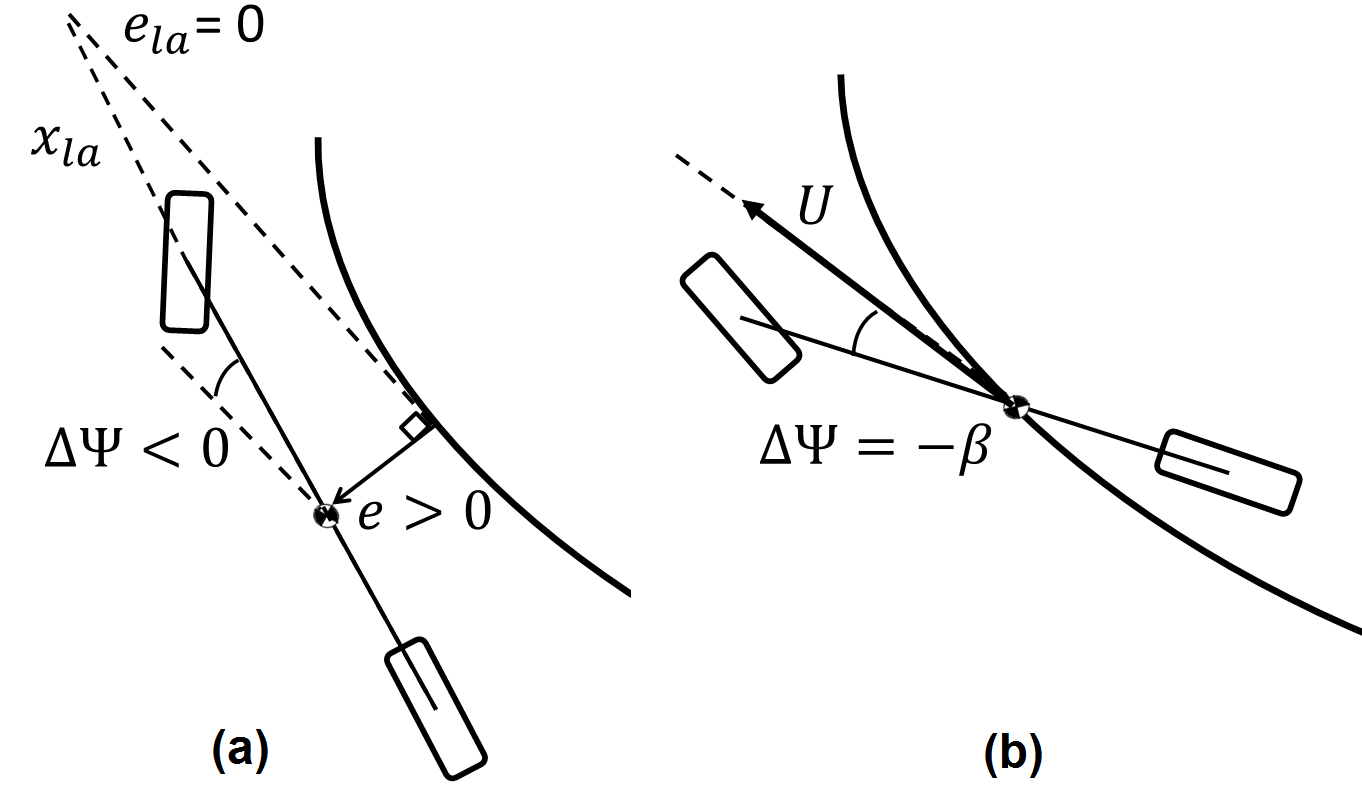
\includegraphics[width=0.65\columnwidth]{figures/SSerror.png}
\caption{(a) Steady-state cornering where vehicle has lateral error but no lookahead error. (b) Zero steady-state lateral deviation requires vehicle velocity vector
to be tangent to path.}
\label{fig:SSerror}
\end{figure}
 
% % % % % % % end figure % % % % % % %

%=======================================================================
\section{Incorporating Sideslip-Path Tangency into Steering Feedback}
\label{sec:betafb}

An interesting observation from Fig.~\ref{fig:linError} is that the steady-state path deviation
 is zero at a vehicle speed of around $U_\mathrm{x}$=20 m/s for the linear model and $U_\mathrm{x}$=17 m/s for the nonlinear model. 
 At these speeds, the steady-state vehicle sideslip is predicted to be zero as well, 
and the vehicle heading $\Psi$ naturally becomes tangent to the desired path heading. 

This observation motivates a second form of lookahead feedback where the feedback objective is to maintain the 
vehicle velocity vector $U$ tangent to the desired path, as shown in Fig.~\ref{fig:SSerror}(b). Since
 $U=\Psi+\beta$, the resulting control law is:
 
 
\begin{subequations}
\label{eqn:vveq}
\begin{align}
        \delta_\mathrm{FB} & = -k_\mathrm{P} (e+x_\mathrm{LA} (U-\Psi_\mathrm{r} ) ) \\
                           & =  -k_\mathrm{P} (e+x_\mathrm{LA} (\Psi+\beta-\Psi_\mathrm{r} )) \\
						   & = -k_\mathrm{P}(e+x_{LA}(\Delta\Psi+\beta))
\end{align}
\end{subequations}
 where $\Psi_\mathrm{r}$ is the heading of the desired vehicle path at a given point. The modified control law can be modeled by reformulating the matrix $A$ in (\ref{eqn:Amatrix}) as:
 
\begin{equation}
\label{eqn:Amatrix2}
A  = 
 \begin{bmatrix}
  0 & U_\mathrm{x} & 0 & U_\mathrm{x} \\
  0 & 0 & 1 & 0 \\
  \frac{-ak_\mathrm{P} C_\mathrm{F}}{I_\mathrm{z}}  & \frac{-ak_\mathrm{P}x_{LA}C_\mathrm{F}}{I_\mathrm{z}}  & \frac{-a^2C_\mathrm{F}-b^2C_\mathrm{R}}{U_\mathrm{x}I_\mathrm{z}} & \frac{bC_\mathrm{R} - aC_\mathrm{F}(1-ak_\mathrm{P}x_\mathrm{LA}) }{I_\mathrm{z}}  \\
  \frac{-k_\mathrm{P}C_\mathrm{F}}{mU_\mathrm{x}}  & \frac{-k_\mathrm{P}x_{LA}C_\mathrm{F}}{mU_\mathrm{x}}  & \frac{-aC_\mathrm{F}-bC_\mathrm{R}}{mU_\mathrm{x}^2}-1 & \frac{-(C_\mathrm{F}(1+k_\mathrm{P}x_\mathrm{LA}) + C_\mathrm{R})}{mU_\mathrm{x}}
 \end{bmatrix}
 \end{equation}
 
\begin{figure}[h]
\centering
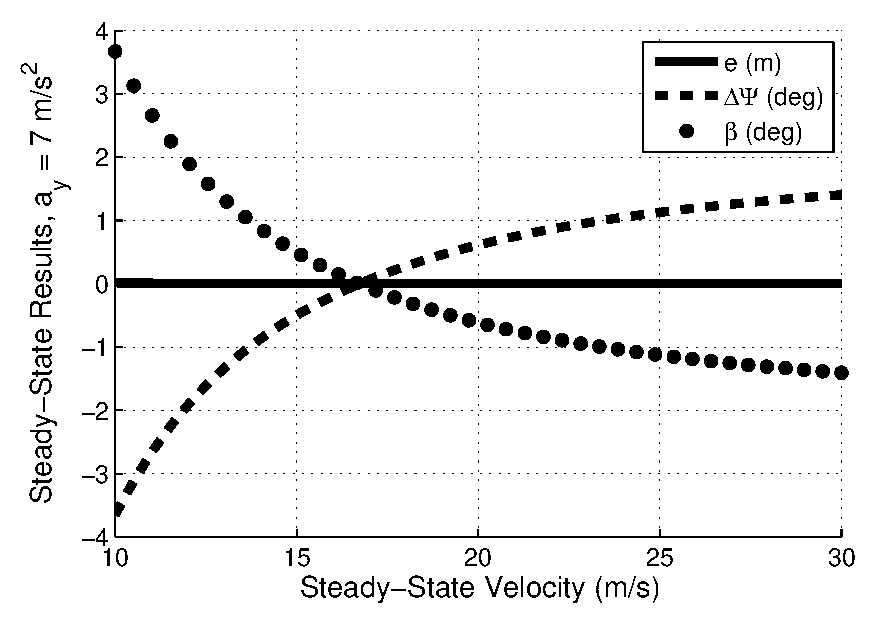
\includegraphics[width=.55\columnwidth]{figures/LinearErrorPlotBeta.eps}
\caption{Steady-state simulation results with sideslip added to feedback control, using the nonlinear vehicle model with fixed lateral acceleration of 7 $\mathrm{m/s^2}$.}
\label{fig:linError2}
\end{figure} 
 
Note that (\ref{eqn:Amatrix2}) is equal to (\ref{eqn:Amatrix}b) with the exception of the last column. Fig.~\ref{fig:linError2}
shows the resulting steady-state behavior, and indicates that lateral error $e$ settles to
zero for all velocities. 

However, the disadvantage of directly adding vehicle sideslip 
into the feedback control is reduced stability margins. One method of observing the relative stability benefits of lookahead feedback is to draw a 
root locus plot of the closed-loop steering system pole locations as a function of vehicle speed. Closed-loop eigenvalues of (\ref{eqn:Amatrix}b) and (\ref{eqn:Amatrix2})
are plotted in Fig.~\ref{fig:rLocusPlot} as a function of increasing vehicle speed from 5 m/s to 25 m/s. The results indicate that the closed-loop steering response
is well-damped ($\zeta =$ .9 at a vehicle speed of 25 m/s) with the original lookahead feedback controller. However, when, the steering feedback acts to 
keep the vehicle sideslip tangent to the desired path via (\ref{eqn:vveq}), the closed-loop steering response becomes highly underdamped 
($\zeta$ = .2 at $U_x$ = 25 m/s).  

\begin{figure}[h]
\centering
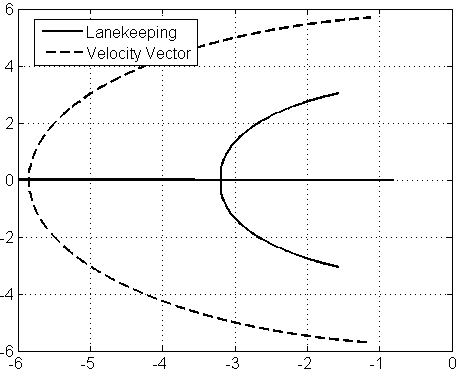
\includegraphics[width=.55\columnwidth]{figures/rLocus.eps}
\caption{Closed-loop pole locations for steering system as vehicle speed is varied from 5 to 25 m/s. Damping ratio $\zeta$ and natural
frequency $\omega_n$ are shown for $U_\mathrm{x}$ = 25.}
\label{fig:rLocusPlot}
\end{figure}

Note that the results shown in Fig.~\ref{fig:rLocusPlot} are for a single vehicle and controller parameterization (see Table 1). 
In general, the reduction in stability margin will vary significantly depending on the vehicle understeer gradient and steering controller gains, namely
the lookahead distance. Fig.~\ref{fig:VcrPlot} shows the critical speed $V_\mathrm{cr}$, beyond which the closed-loop 
steering system becomes unstable, for neutral, understeering, and oversteering configurations as a function of $x_\mathrm{LA}$.   

\begin{figure}[h]
\centering
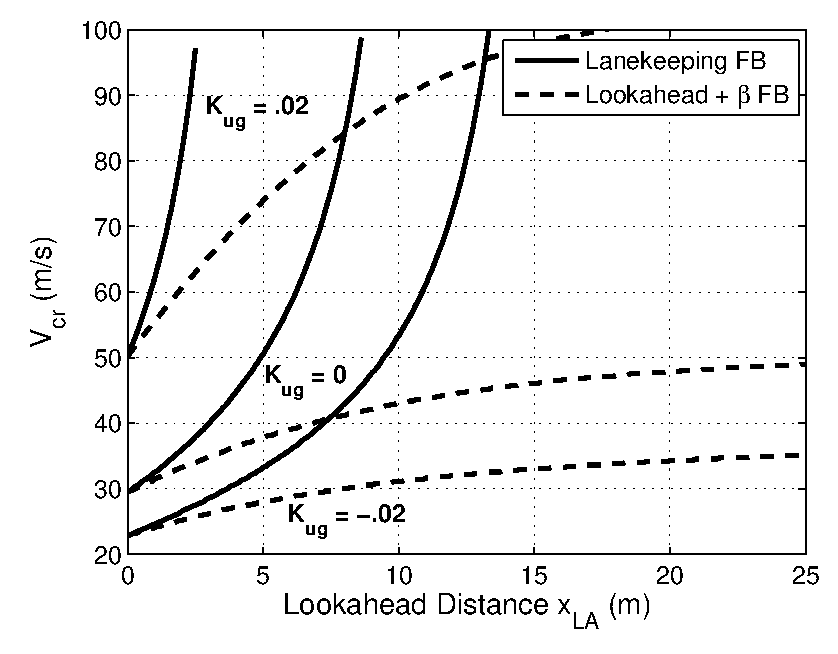
\includegraphics[width=.75\columnwidth]{figures/VcrPlot.eps}
\caption{Maximum speed for closed-loop stability for the original lookahead feedback and the modified feedback with sideslip tracking. Results are based on
eigenvalue computations of the $A$ matrix of the linear vehicle model.}
\label{fig:VcrPlot}
\end{figure}

For an understeering vehicle, lookahead feedback is always stable as long
as the lookahead point $x_\mathrm{LA}$ is above a certain critical value (a conclusion derived in \cite{rosseter}). Even in situations where the vehicle is in a 
neutral steer or oversteer configuration, the critical speed for closed-loop stability increases rapidly with lookahead distance. A different trend is present when
sideslip tracking is added to the steering feedback. Fig.~\ref{fig:VcrPlot} shows that the critical speeds for 
stability increase very slowly as a function of lookahead distance.

\section{Incorporating Sideslip Information Into Steering Feedforward}
\label{sec:goodFFW}
 
 Given the trade-off between path tracking and stability when sideslip-path alignment is enforced via feedback, a promising approach
 is to replace vehicle sideslip  $\beta$ in (\ref{eqn:vveq}) with the predicted steady-state sideslip value $\beta_\mathrm{ss}$ 
 for a given vehicle speed and curvature. 

The rear tire slip for a fixed track vehicle, assuming small angles, is given by 
\begin{equation}
\alpha_\mathrm{r} = \beta - \frac{br}{U_\mathrm{x}}
\end{equation} 

At steady-state, $\alpha_\mathrm{r}=\alpha_\mathrm{r}^\mathrm{FFW}$ from (\ref{eqn:steadyffw}) and $r_\mathrm{ss}=\kappa U_\mathrm{x}$, yielding the following feedback control law:

\begin{subequations}
\begin{align}
\label{eqn:betass}
\delta_\mathrm{FB} &=-k_\mathrm{P} (e+x_\mathrm{LA} (\Delta\Psi+\beta_\mathrm{ss})) \\
\beta_\mathrm{ss}  &= \alpha_\mathrm{r}^\mathrm{FFW} + b\kappa
\end{align}
\end{subequations}

The effect of this change is to remove the steering controller's dependence on \textit{real-time} sideslip information. The steering
controller will now act to align the vehicle's predicted \textit{steady-state} sideslip along the desired path. Since the controller no
longer has feedback on vehicle sideslip, the state matrix equation $A$ for the closed-loop system dynamics is now 
once again given by (\ref{eqn:Amatrix}b), which was shown to have desirable stability
properties as a function of $K_\mathrm{ug}$ and $x_\mathrm{LA}$ (Fig.~\ref{fig:VcrPlot}). The sideslip now affects the vehicle
path tracking dynamics through the feedforward path, since the predicted steady-state sideslip $\beta_{ss}$ depends only on the
desired speed $U_x$ and curvature $\kappa$ as well as the feedforward tire model. The $B$ matrix in (\ref{eqn:Amatrix}) now becomes: 

\begin{subequations}
\label{eqn:newB}
\begin{align}
	B &=[0 \hspace{2 mm} -U_\mathrm{x} \hspace{3 mm} \frac{a C_\mathrm{F} (G_\mathrm{FFW}+G_\beta)}{I_\mathrm{z}} \hspace{3 mm}  \frac{C_\mathrm{F} (G_\mathrm{FFW}+G_\beta)}{mU_\mathrm{x}}]^T \\
	G_\beta &= U_\mathrm{x}^2\frac{ma}{L}\frac{k_\mathrm{P}x_\mathrm{LA}}{C_\mathrm{R}}
\end{align}
\end{subequations}

Assuming perfect knowledge of the feedforward tire model, the resulting steady-state lateral path deviation will be zero at all vehicle speeds,
as shown in Fig.~\ref{fig:linError2}. However, error in the feedforward tire model will result in steady-state lateral path deviation.
The effect of incorporating steady-state sideslip into the feedforward control is shown in Fig.~\ref{fig:ffwplot}. The feedforward
steering command $\delta_\mathrm{FFW}$ as a function of path curvature and vehicle speed is plotted both for the original feedforward control law (\ref{eqn:Amatrix}c) as well as the sideslip-incorporating
feedforward command (\ref{eqn:newB}). 

\begin{figure}[h]
\centering
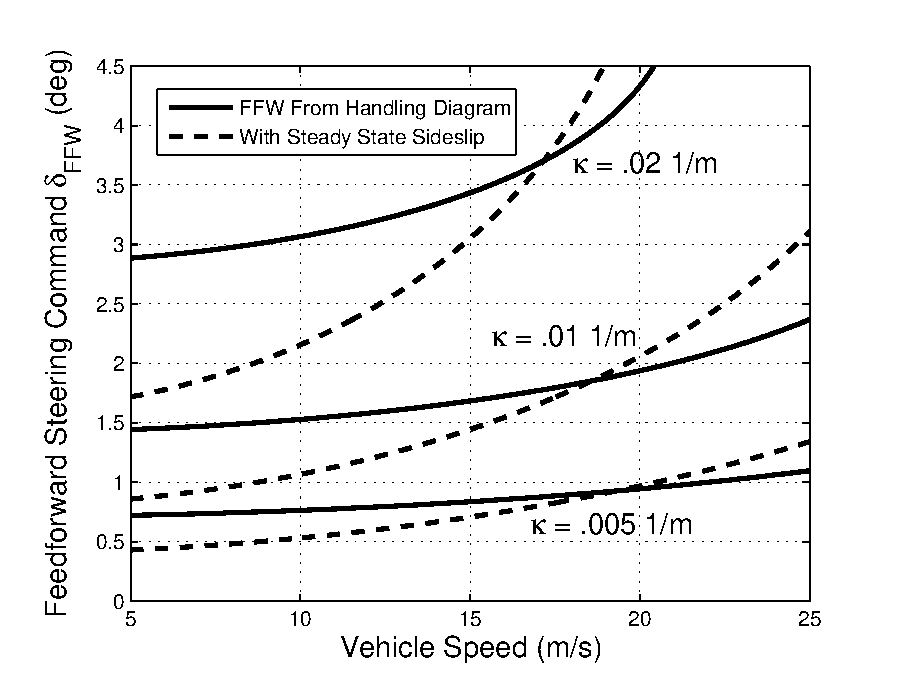
\includegraphics[width=.75\columnwidth]{figures/FFWplot.eps}
\caption{Effect of incorporating sideslip behavior into feedforward steering command $\delta_\mathrm{FFW}$, as a function of 
vehicle speed and desired path curvature.}
\label{fig:ffwplot}
\end{figure}

\section{Experimental Results}

\subsection{Experimental Setup}

Experimental data was collected on an Audi TTS equipped 
with an electronic power steering motor for autonomous steering and active brake booster and throttle by wire for
longitudinal control (Fig.~\ref{fig:shelleyPic}).
An integrated Differential Global Positioning System (DGPS) and Inertial Measurement Unit (IMU) is used to obtain
 global vehicle states. 
A map-matching algorithm synthesizes information 
from the GPS to determine the vehicle's position along the desired path and obtain the lateral path deviation
$e$ and vehicle heading error $\Delta\Psi$. 
The controller operates at 200 Hz. 
Vehicle parameters for the Audi test vehicle and the lookahead feedback gains are presented in Table \ref{tb:params}.


\begin{figure}[h]
\centering
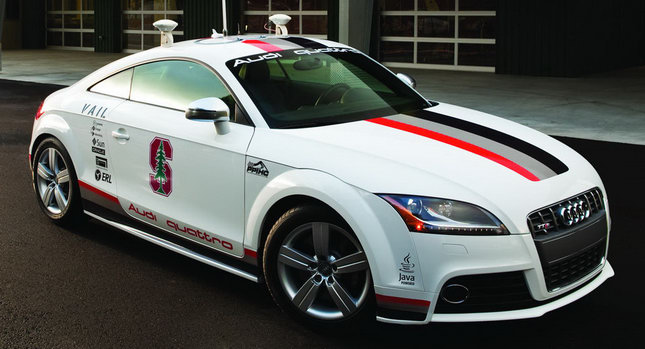
\includegraphics[width=.75\columnwidth]{figures/experimentInfo.jpg}
\caption{Audi TTS used for experimental validation.}
\label{fig:shelleyPic}
\end{figure}
 
\begin{table}[h]
\small
\begin{center}
\caption{Vehicle Parameters}\label{tb:params}
\begin{tabular}{lccc}
Parameter & Symbol & Value & Units \\\hline
Vehicle mass & $m$ & 1500 & kg \\
Yaw moment of inertia & $I_z$ & 2250 & $\mathrm{kg \cdot m}^2$\\
Front axle to CG & $a$ & 1.04 & m\\
Rear axle to CG & $b$ & 1.42 & m\\
Front cornering stiffness & $\mathrm{C}_\mathrm{F}$ & 160 & $\mathrm{kN \cdot rad}^{-1}$ \\
Rear cornering stiffness & $\mathrm{C}_\mathrm{R}$ & 180 & $\mathrm{kN \cdot rad}^{-1}$ \\
Lookahead Distance		 & $x_\mathrm{LA}$         & 14.2 & $\mathrm{m}$ \\
Lookahead Gain         & $k_\mathrm{LK}$         & .053 & $\mathrm{rad/m}$ \\\hline
\end{tabular}
\end{center}
\end{table}

The site for data collection was a 3.1 mile paved racing circuit (friction coefficient $\mu$ = 1) at Thunderhill Raceway Park in Willows, CA.
Fig.~\ref{fig:thPic} shows an overhead view of the race track as well as the desired racing line. The desired racing
line is parameterized as a curvature profile $\kappa(s)$ that varies with distance along the path. The curvature
profile associated with the racing line is shown in Fig.~\ref{fig:traj}
along with a typical longitudinal velocity profile $U_\mathrm{x}$ from the path planner \cite{theodosis}.

\begin{figure}[h]
\centering
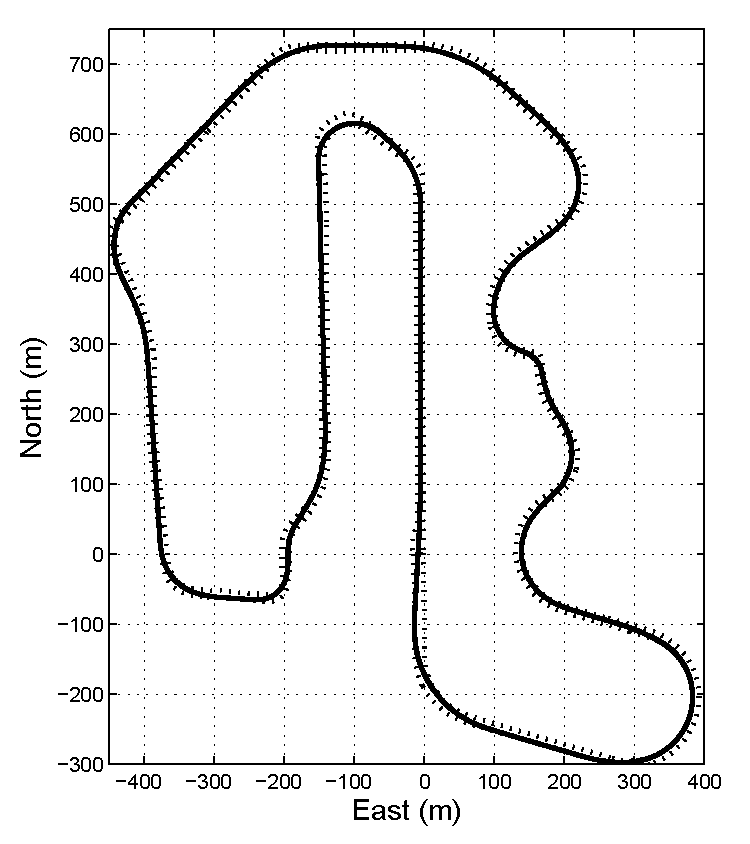
\includegraphics[width=.75\columnwidth]{figures/racingLine.eps}
\caption{Overhead view of path planner output for steering controller to follow.}
\label{fig:thPic}
\end{figure}

\begin{figure}[h]
\centering
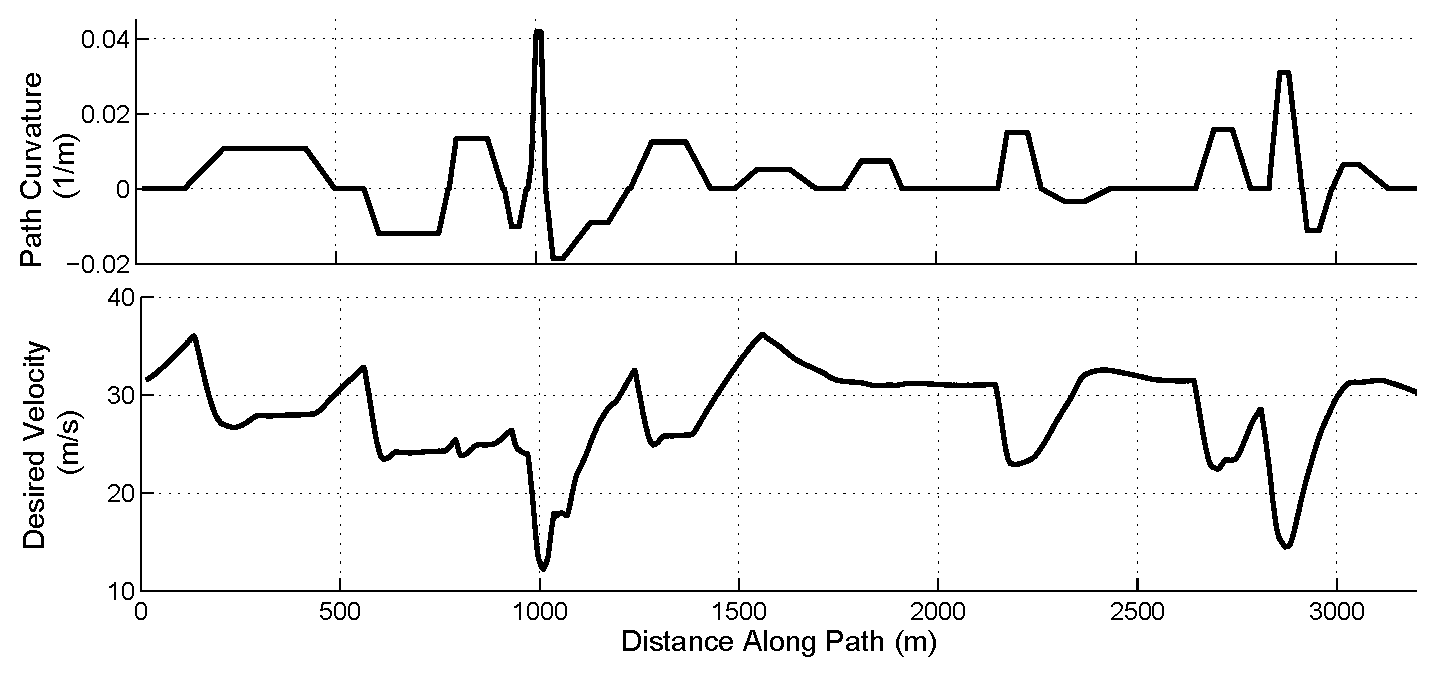
\includegraphics[width=.8\columnwidth]{figures/traj.eps}
\caption{Curvature and velocity profile inputs for steering controller as a function of distance along racing line.}
\label{fig:traj}
\end{figure}

\subsection{Experimental Testing of Sideslip Feedback Controller}

The steering feedback controller with sideslip-path tangency presented in Section \ref{sec:betafb} offers very low path tracking error, but at the
expense of reduced stability margins. To test this controller safely at the limits of handling, experimental data was collected on a
constant radius turn in an open parking lot at two constant speeds. The results of this test are shown in Fig.~\ref{fig:wipeout}. As a baseline, the
feedback controller with sideslip (\ref{eqn:vveq}) from Section \ref{sec:betafb} is compared to the original lookahead feedback controller (\ref{eqn:lookahead}). 
The feedforward steering based on the nonlinear handling diagram (\ref{eqn:steadyffw}) is used in both cases. 

For the case where the speed is 10 m/s, the resulting steady-state acceleration is 7 $\mathrm{m/s^2}$, and both steering controllers maintain stability of the vehicle. 
In addition, incorporating sideslip-path tangency into the feedback control law results in significantly lower path tracking errors compared to the baseline
lookahead feedback controller. However, when the speed is increased to 13 m/s, the resulting steady-state lateral acceleration is 9 $\mathrm{m/s^2}$,
and the sideslip feedback controller becomes unstable and goes into a spin, as demonstrated by the plots of yaw rate and sideslip. For the same conditions,
the baseline lookahead controller remains stable. The issue with the sideslip feedback controller is shown in the plot of vehicle sideslip and heading
error. As the vehicle heading error decreases and becomes unstable around $s = $ 170 m, the feedback controller does not intervene because the
 vehicle's velocity vector remains tangent to the path (i.e. $\Delta\Psi + \beta =$ 0). A counter steering action is finally provided at $s = $ 190 m, but at this point the vehicle
has already spun out.

\begin{figure}[h]
\centering
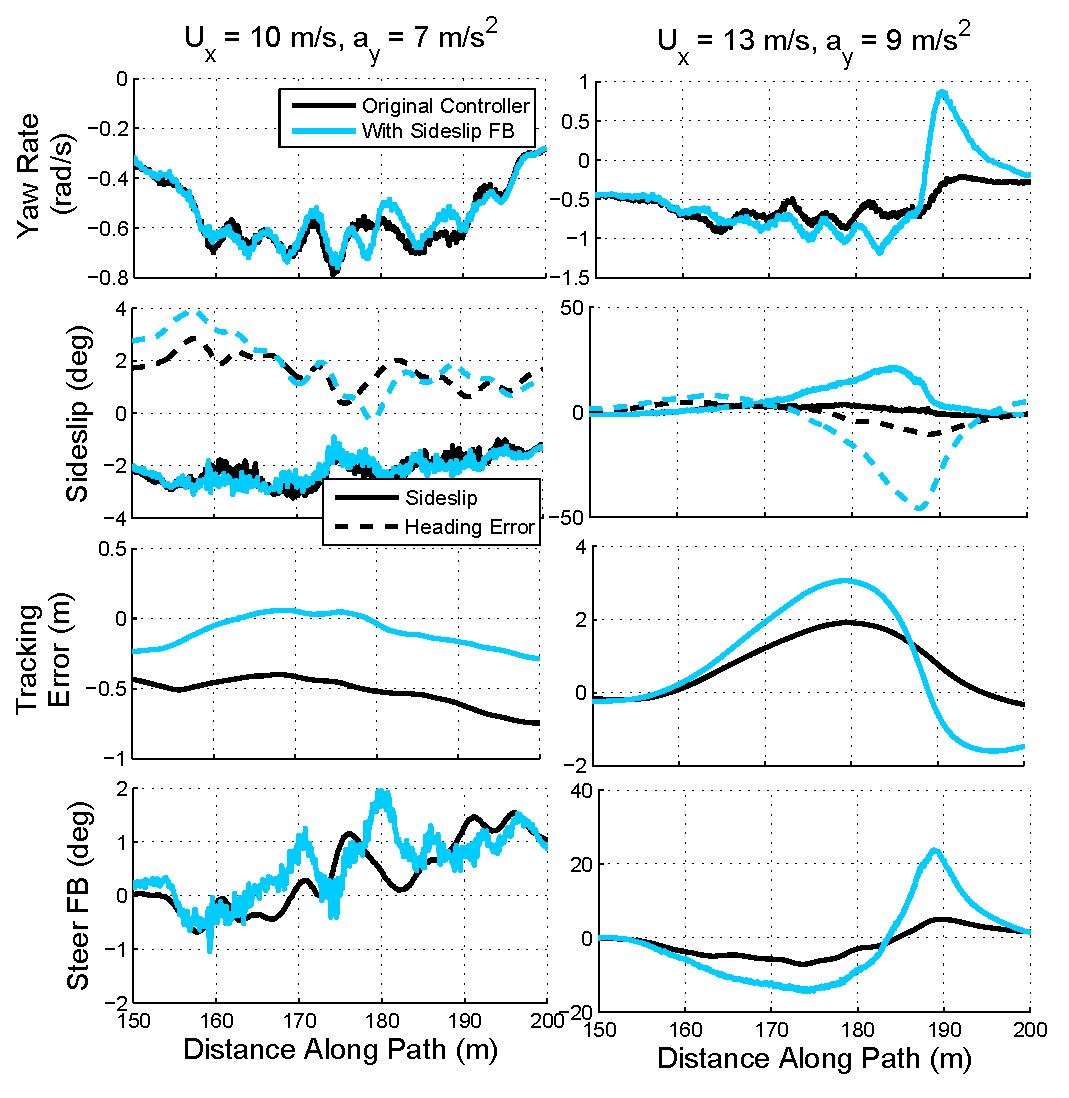
\includegraphics[width=.9\columnwidth]{figures/wipeout.eps}
\caption{Parking lot test for constant radius turning at 10 m/s and 13 m/s. Resulting steady-state accelerations are 7 $\mathrm{m/s^2}$ and 9
$\mathrm{m/s^2}$. Steering feedback with sideslip is compared to original lookahead steering controller.}
\label{fig:wipeout}
\end{figure}




\subsection{Experimental Data from Racetrack}

Fig.~\ref{fig:betaComparison} shows experimental data taken over a 3 km subset of the entire racetrack,
excluding portions of the course where there is little vehicle cornering. The experimental data is plotted for two separate steering
controllers. The first controller is the `baseline' controller described in Section \ref{sec:controller}, with the
steering feedback provided by the lookahead system and the feedforward steering given by the steady-state handling diagram. The second controller uses the same lookahead feedback, but incorporates the steady-state sideslip
behavior into the feedforward steering to align the vehicle's velocity vector with the path heading (Section \ref{sec:goodFFW}).
Note that the controller where real-time sideslip was incorporated into the steering feedback (Section \ref{sec:betafb}) was not tested, as there is a high likelihood
of vehicle instability near the limits of handling given the results from the previous parking lot test. The same longitudinal controller is used for both cases in order to
 brake into the entry of turns and accelerate out of turn exits. For this lap, the peak longitudinal deceleration is -8 $\mathrm{m/s^2}$ and
 peak lateral acceleration is 8 $\mathrm{m/s^2}$.
 
 
\begin{figure}[h]
\centering
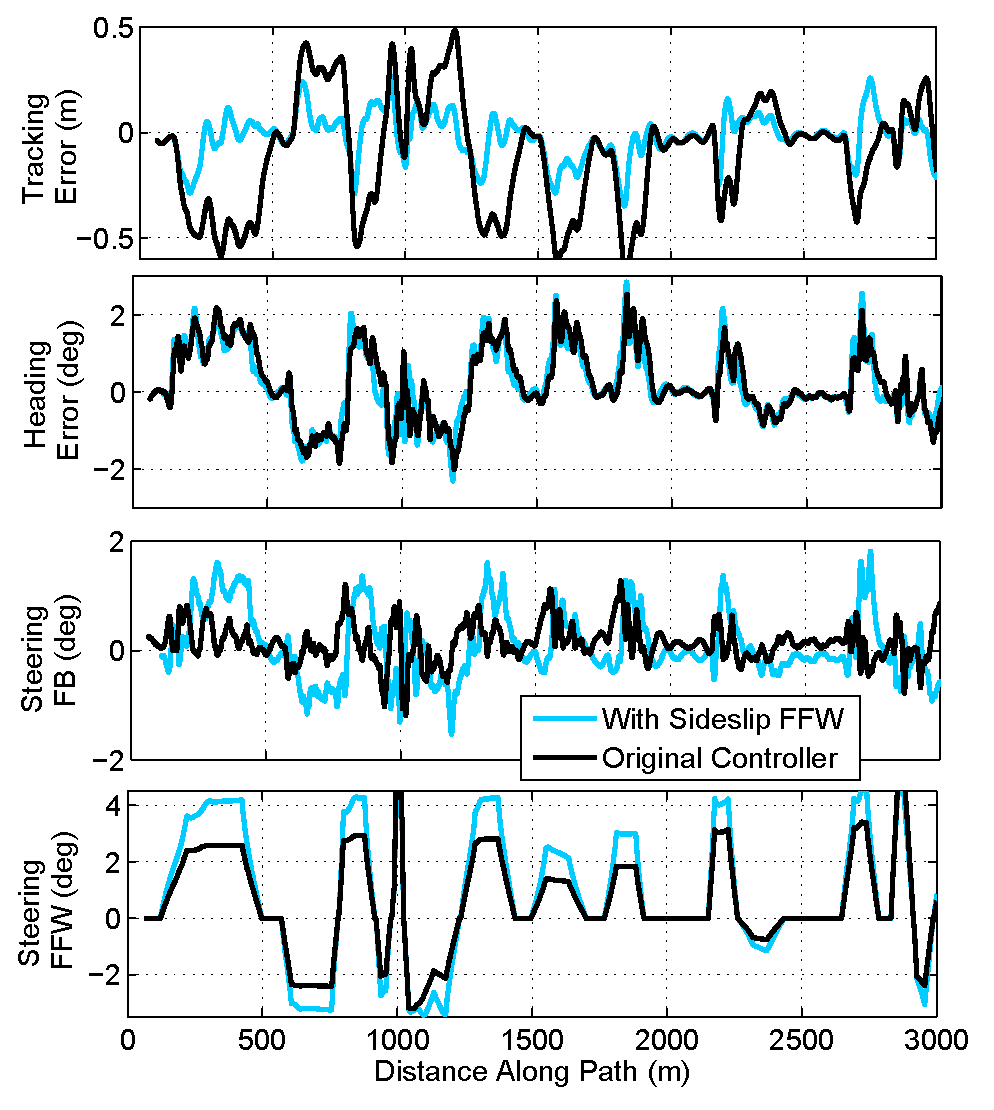
\includegraphics[width=\columnwidth]{figures/betaCompensation.eps}
\caption{Experimental data with combined acceleration magnitude 8 $\mathrm{m/s^2}$ over 3 km stretch of Thunderhill Raceway Park.}
\label{fig:betaComparison}
\end{figure}


The results in Fig.~\ref{fig:betaComparison} show that lateral path deviation $e$ is reduced when incorporating 
steady-state sideslip in the feedforward control law. This confirms the expected results from the analysis performed in Sections \ref{sec:predSS}
and \ref{sec:goodFFW}. Note that while the lateral path deviation is smaller, the levels of vehicle heading error $\Delta\Psi$ remain roughly the
same. This matches the predicted result in Fig.~\ref{fig:linError2}. The steering controller will align the vehicle's
velocity vector with the path, not the vehicle's heading, and due to a vehicle's tendency to develop a steady-state sideslip angle,
 a non-zero heading error $\Delta\Psi$ is in general necessary for zero steady-state lateral path deviation,
 as shown by the schematic in Fig.~\ref{fig:SSerror}(b).

\begin{figure}[h]
\centering
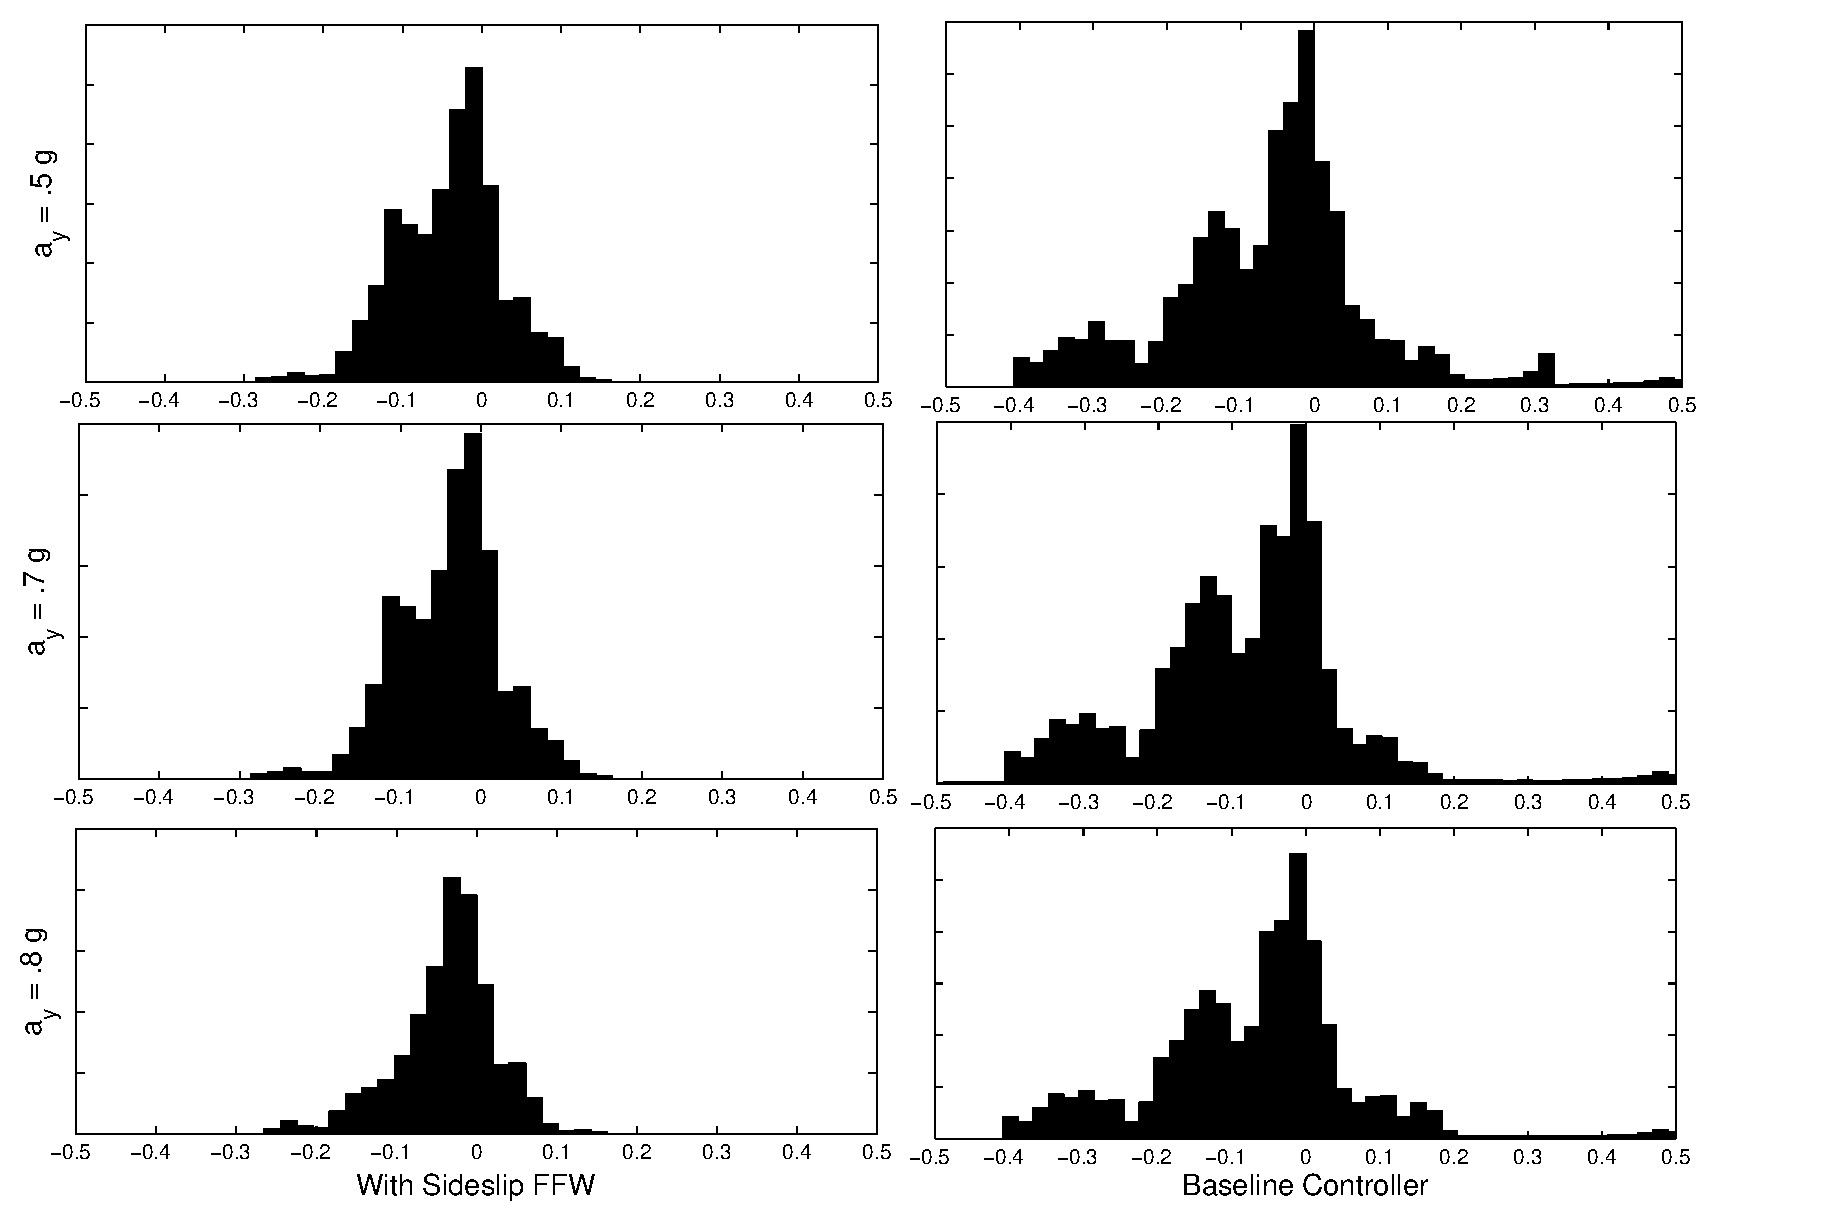
\includegraphics[width=\columnwidth]{figures/errhist.eps}
\caption{Histogram of path tracking error for six laps around the track. Left column represents performance of controller
with feedforward sideslip tracking, and right column is baseline controller with feedforward from
the steady-state handling diagram.}
\label{fig:errhist}
\end{figure}

For a better sense of the improvement in lateral path deviation, Fig.~\ref{fig:errhist} shows histogram plots of the lateral tracking
error $e$ for both controllers over three laps taken at varying levels of peak lateral acceleration. The baseline controller keeps the vehicle within 0.5 meters
 on either side of the desired path, with a large
amount of variation in the resulting histogram. An interesting observation is that the 
histogram is not symmetric. In general, the raceway has more left turns than right turns, and as Fig.~\ref{fig:linError} indicates, at
high speeds the baseline controller will track toward the outside of the turn. This tendency is manifested experimentally in the asymmetric nature
of the histograms. The histograms for the improved controller show a much tighter distribution on the lateral path tracking 
error. The path tracking error generally remains within 10-15 cm on either side of the lane boundary and contains less of a bias towards tracking
on the outside of turns.  

\begin{figure}[h]
\centering
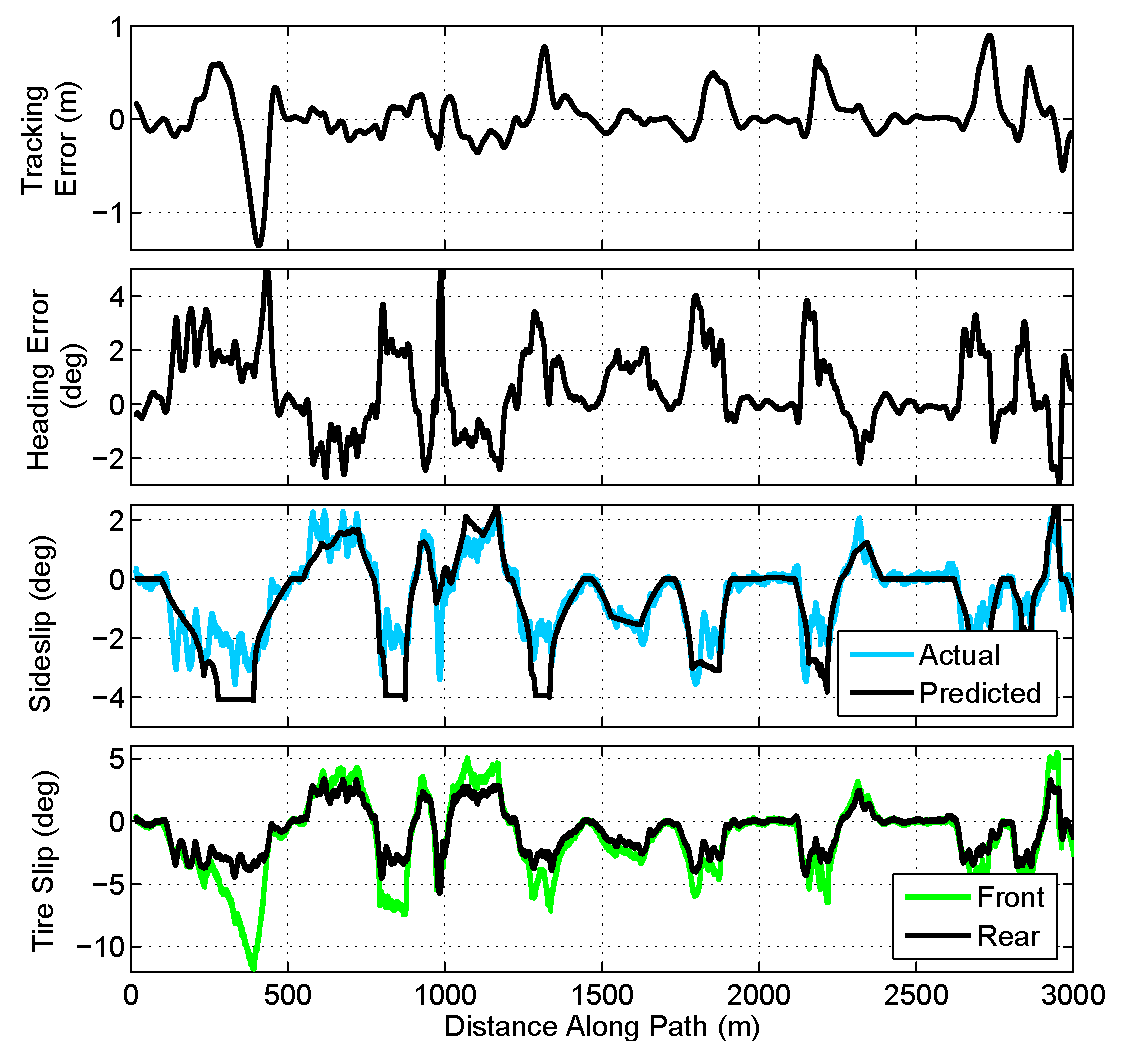
\includegraphics[width=\columnwidth]{figures/atTheLimits.eps}
\caption{Experimental data with combined acceleration magnitude 9.5 $\mathrm{m/s^2}$ over 3 km stretch of Thunderhill Raceway Park.}
\label{fig:atTheLimits}
\end{figure}

As the lateral acceleration increases beyond 0.8 g and the vehicle approaches the handling limits, the steering controller
remains stable and well-damped, although the tracking performance begins to degrade. Fig.~\ref{fig:atTheLimits} shows experimental
data for a lap around Thunderhill Raceway park with peak lateral and longitudinal accelerations of 0.95 g. At several points along the
track, the tracking error increases above 0.5 m, significantly higher than the levels of path deviation seen at 0.8 g of vehicle acceleration.
The reasons for this are three-fold. 

First, the sharp drop in front tire slip from $s$ = 300 - 400 meters indicates that the 
 lateral force demand for the front tires has exceeded the available friction at that region of the track. As a result, the vehicle
 understeers heavily and tracks well to the outside of the left-hand turn, resulting in a large negative tracking error.
At this point, there is nothing the steering controller can do to bring the vehicle back to the desired path, and the vehicle must alter its
desired trajectory to become less aggressive, either by slowing down or reducing the turn curvature. Second, the steady-state feedforward controller requires an accurate estimate of the vehicle parameters in order to estimate
the steady-state sideslip in (\ref{eqn:betass}). From $s$ = 700-800, 1300-1400, 1800-1900, and 2200-2300 meters along the track, there are observable
discrepancies between the predicted feedforward sideslip and the actual vehicle sideslip, as measured by the GPS-INS. Not surprisingly,
this plant-model mismatch results in significant path tracking errors at those portions of the racing circuit. Finally, the feedforward
model in (\ref{eqn:betass}) assumes steady-state conditions. As the vehicle approaches the limits of handling, transient vehicle
dynamics can result in larger path deviations as well.

Future work will focus on reducing the latter two sources of error by gradually learning a better feedforward model of the
vehicle dynamics over time. For situations where a vehicle repeats a given trajectory multiple times, iterative learning control (ILC)
is a promising technique for refining the feedforward input to improve the reference tracking performance of the controller. Additionally, online estimation
approaches can also be used to gradually improve knowledge of difficult-to-measure parameters such as friction and vehicle cornering
stiffness.

%=======================================================================
\section{Conclusion}

This paper describes the design of a feedback-feedforward controller capable of path tracking at the limits of handling. Desirable
 path tracking behavior occurs when the vehicle sideslip is aligned
with the desired path heading. However, directly incorporating this behavior into a feedback steering control law results in 
a closed-loop controller with poor stability margins. 
A better approach for combined path tracking and stability is to align the steady-state vehicle sideslip 
with the desired path heading through the feedforward steering command. 
This enables improved path tracking while maintaining the robust stability properties of lookahead steering feedback. Results from a histogram
analysis quantitatively indicate that the improved feedforward command reduces lateral path deviation by more than fifty percent.
One potential drawback is that this feedforward approach is sensitive to vehicle model uncertainty, especially at the physical
limits of handling where transient dynamics become prevalent. Future work will seek to use methods such as iterative learning control
or online parameter estimation to improve the feedforward vehicle model and eliminate undesirable transient dynamics. \\

\subsection{Acknowledgements}

The authors would like to thank Joe Funke, Paul Theodosis, Krisada Kritayakirana, John Kegelman, and Steve Erlien of the Dynamic Design Lab at Stanford University, as well as Rob Simpson and Rick Keiner of the Audi Electronics Research Lab.

\subsection{Funding}

This research is supported by the National Science Foundation Graduate Research Fellowship Program (GRFP) as well as a Stanford Graduate Fellowship (SGF). 


\bibliographystyle{nVSD}
\bibliography{Bibliography}


\end{document}
